% This work is made available under the terms of the
% Creative Commons Attribution-ShareAlike 4.0 license,
% http://creativecommons.org/licenses/by-sa/4.0/.
%
% Version: $Revision$

\chapter{Tools}

\section{Append datasets}

If you have datasets with the same structure, i.e., exactly the same
attributes, then you can use the \textit{Append datasets} tool to combine
them into a single, large dataset.

The screenshot in Figure \ref{dataset-compatibility} shows the wizard
interface that guides you through the process.

\begin{figure}[htb]
  \centering
  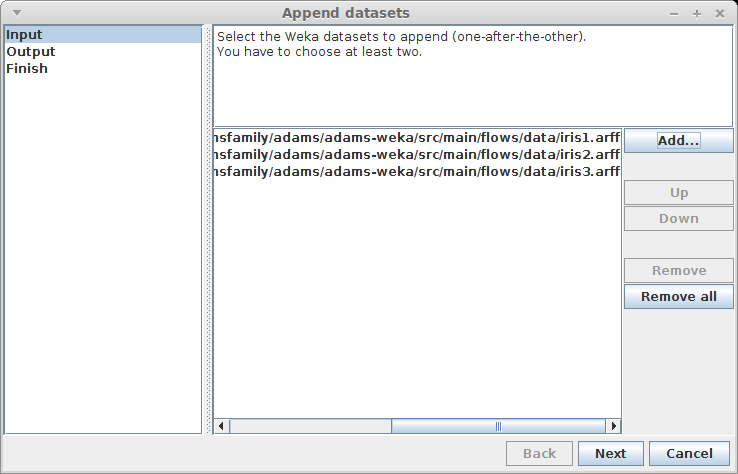
\includegraphics[width=12.0cm]{images/append_datasets.png}
  \caption{Appending datasets wizard.}
  \label{append_datasets}
\end{figure}

\clearpage
\section{Arff viewer}

WEKA's \textit{Arff viewer} is available from the ADAMS menu as well.

\begin{figure}[htb]
  \centering
  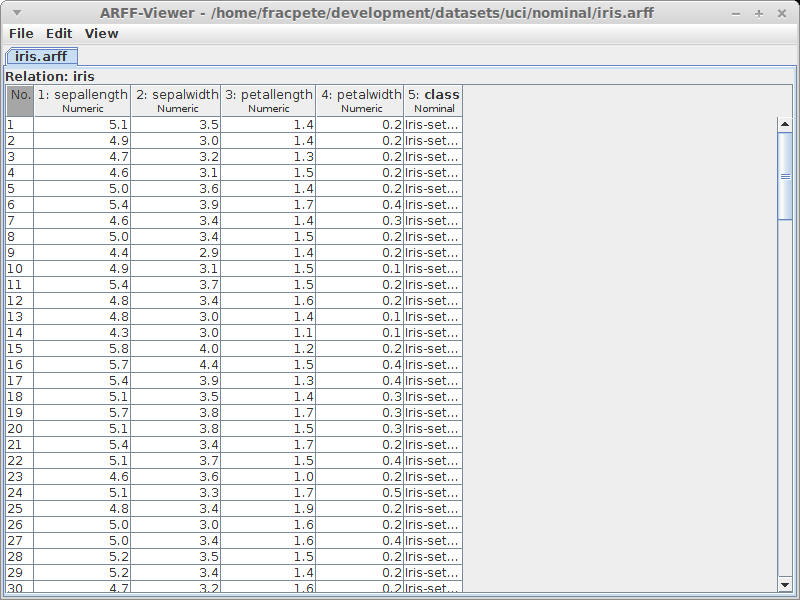
\includegraphics[width=12.0cm]{images/arffviewer.png}
  \caption{WEKA's Arff viewer displaying the iris UCI dataset.}
  \label{arffviewer}
\end{figure}

\clearpage
\section{Batch-filter datasets}

Training and test set are required to have exactly the same structure
in WEKA. If you need to apply a pre-processing filter to both of the
files, it is recommended to use \textit{batch-filtering}. This will
ensure that any statistics that get calculated based on the first
dataset, get applied to second file as well. An example for this is
the dictionary of the \textit{StringToWordVector}: the same word
dictionary needs to be applied to the second file, in order to generate
the same attributes. However, one usually has to resort to the command-line
in order to achieve this, which is rather tedious.

The \textit{Batch-filter datasets} wizard allows you to perform the
batch-filtering conveniently through the GUI:
\begin{tight_itemize}
  \item Select the datasets to filter (see \ref{batchfilter_datasets1})
  \item Configure the filter (see \ref{batchfilter_datasets2})
  \item Select the output directory (see \ref{batchfilter_datasets3})
  \item Info dialog after filtering (see \ref{batchfilter_datasets4})
\end{tight_itemize}

\begin{figure}[htb]
  \centering
  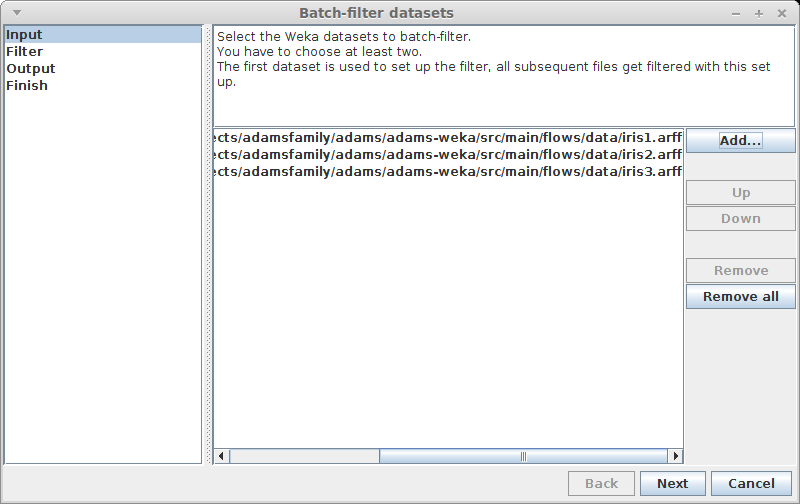
\includegraphics[width=12.0cm]{images/batchfilter_datasets1.png}
  \caption{Selecting input files for batch-filtering.}
  \label{batchfilter_datasets1}
\end{figure}

\begin{figure}[htb]
  \centering
  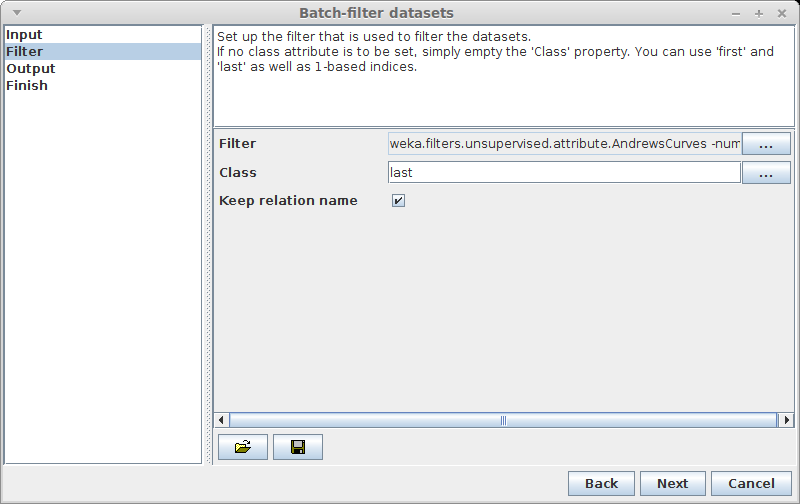
\includegraphics[width=12.0cm]{images/batchfilter_datasets2.png}
  \caption{Configuring the filter.}
  \label{batchfilter_datasets2}
\end{figure}

\begin{figure}[htb]
  \centering
  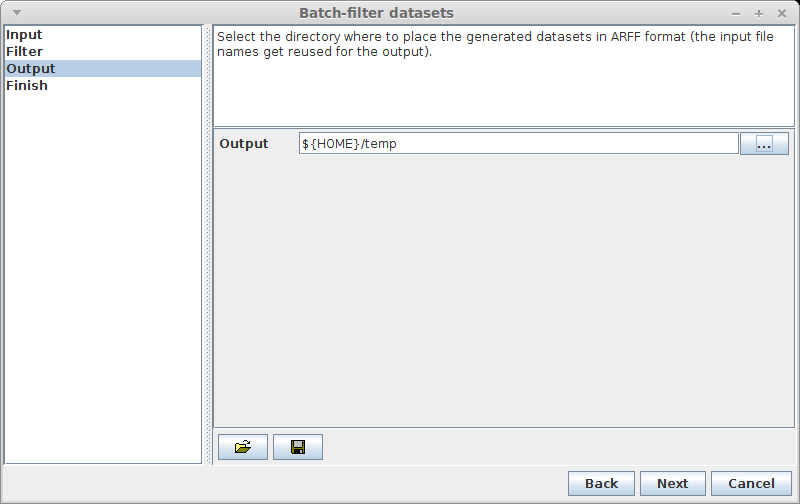
\includegraphics[width=12.0cm]{images/batchfilter_datasets3.png}
  \caption{Selecting the output directory for the filtered datasets.}
  \label{batchfilter_datasets3}
\end{figure}

\begin{figure}[htb]
  \centering
  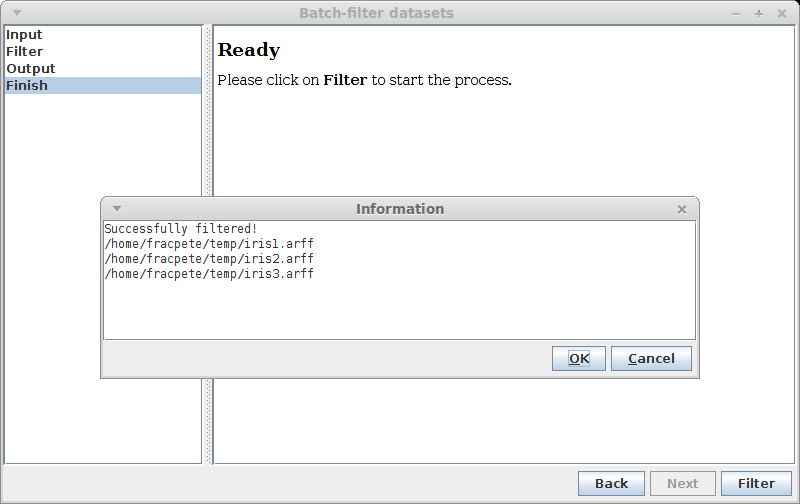
\includegraphics[width=12.0cm]{images/batchfilter_datasets4.png}
  \caption{The dialog when batch-filtering was successful.}
  \label{batchfilter_datasets4}
\end{figure}

\clearpage
\section{BayesNet Editor}
WEKA's \textit{BayesNet Editor} allows you to view and modify Bayesian nets.
Figure \ref{bayesnet_editor} shows an example net loaded.

\begin{figure}[htb]
  \centering
  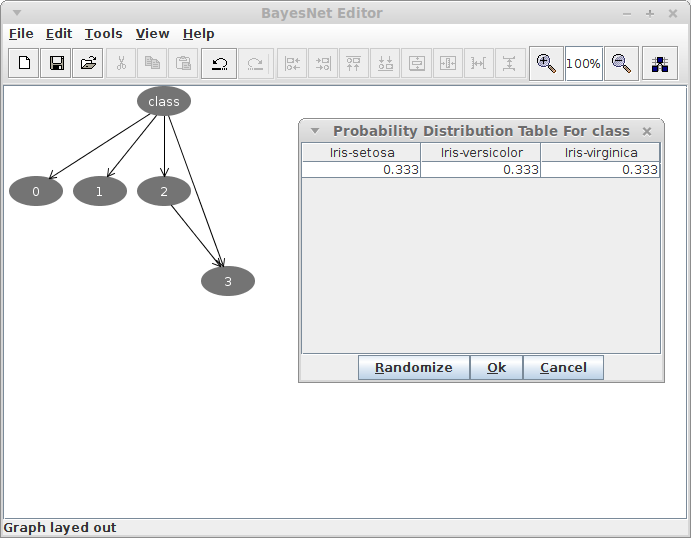
\includegraphics[width=12.0cm]{images/bayesnet_editor.png}
  \caption{BayesNet editor displaying a net.}
  \label{bayesnet_editor}
\end{figure}

\clearpage
\section{Dark Lord}
The \textit{Dark Lord} wizard allows you to set up and monitor a genetic
algorithm that determines the best set of attributes, based on the classifier
and metric you choose to optimize on. The output directory that you define
(see Figure \ref{darklord_setup}), is used to store all the \textit{reduced/optimized}
datasets that improved the metric. The optimization can be paused, resumed or
stopped with the buttons at the bottom right of the view panel (see Figure
\ref{darklord_run}).

\begin{figure}[htb]
  \centering
  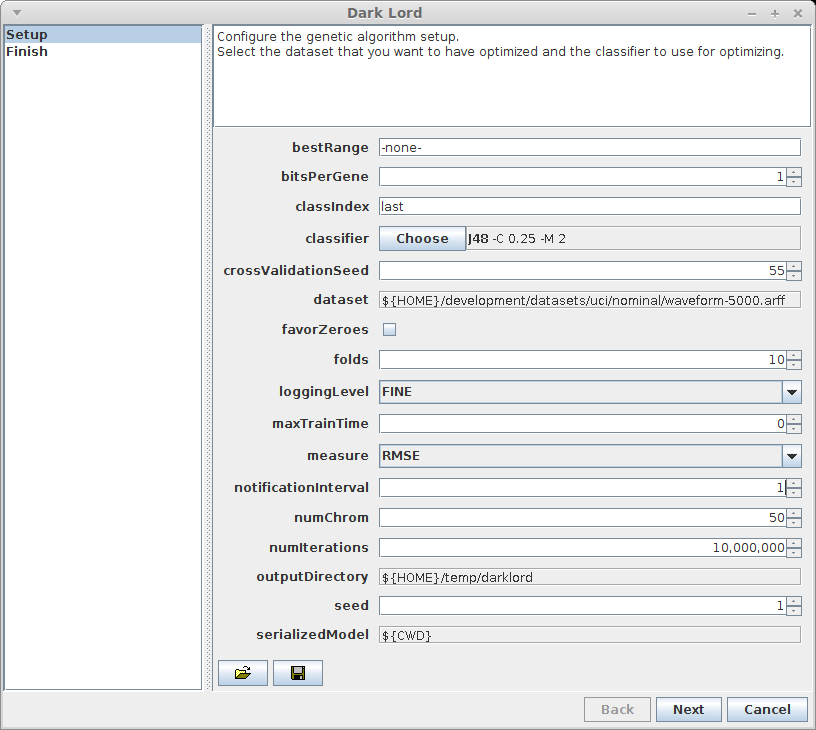
\includegraphics[width=12.0cm]{images/darklord_setup.png}
  \caption{Dark Lord setup.}
  \label{darklord_setup}
\end{figure}

\begin{figure}[htb]
  \centering
  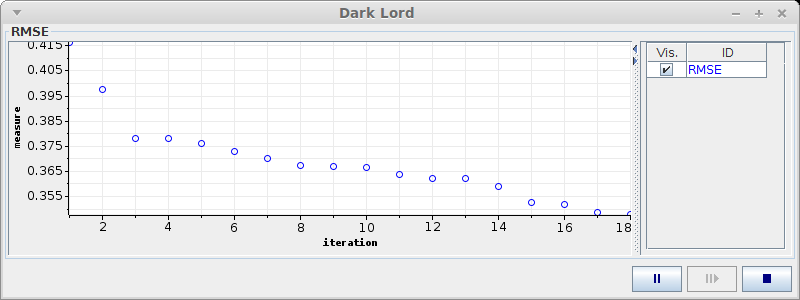
\includegraphics[width=12.0cm]{images/darklord_run.png}
  \caption{Dark Lord run.}
  \label{darklord_run}
\end{figure}

\clearpage
\section{Dataset compatibility}

WEKA requires training and test sets to have the same structure, down to the
same name and order of nominal labels. Rather than relying on the error message
in the Explorer, you can use the \textit{Dataset compatibility} tool to 
quickly check whether two or more datasets are actually compatible.

The screenshot in Figure \ref{dataset-compatibility} shows the output when
comparing two datases, one being the original \textit{anneal} UCI dataset
and the other one a transformed version.

\begin{figure}[htb]
  \centering
  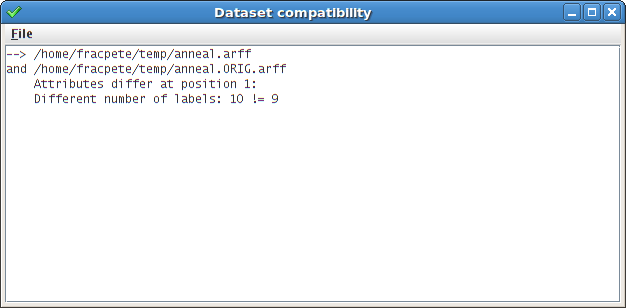
\includegraphics[width=12.0cm]{images/dataset-compatibility.png}
  \caption{Compatibility output for two datasets.}
  \label{dataset-compatibility}
\end{figure}

\clearpage
\section{Explorer}
ADAMS contains an extended version of the WEKA Explorer. The interface uses
menus instead of buttons to declutter the pre-process tab. Also, it keeps track
of the datasets that the user loads, to make re-loading recent files easier.
This saves a lot of time when working with the same files on a frequent basis.
Furthermore, the user can have an arbitrary number of Explorer sessions in the
same window, distinguished by names. Figure \ref{explorerext} shows the new
interface with the drop-down menu in action.

\begin{figure}[htb]
  \centering
  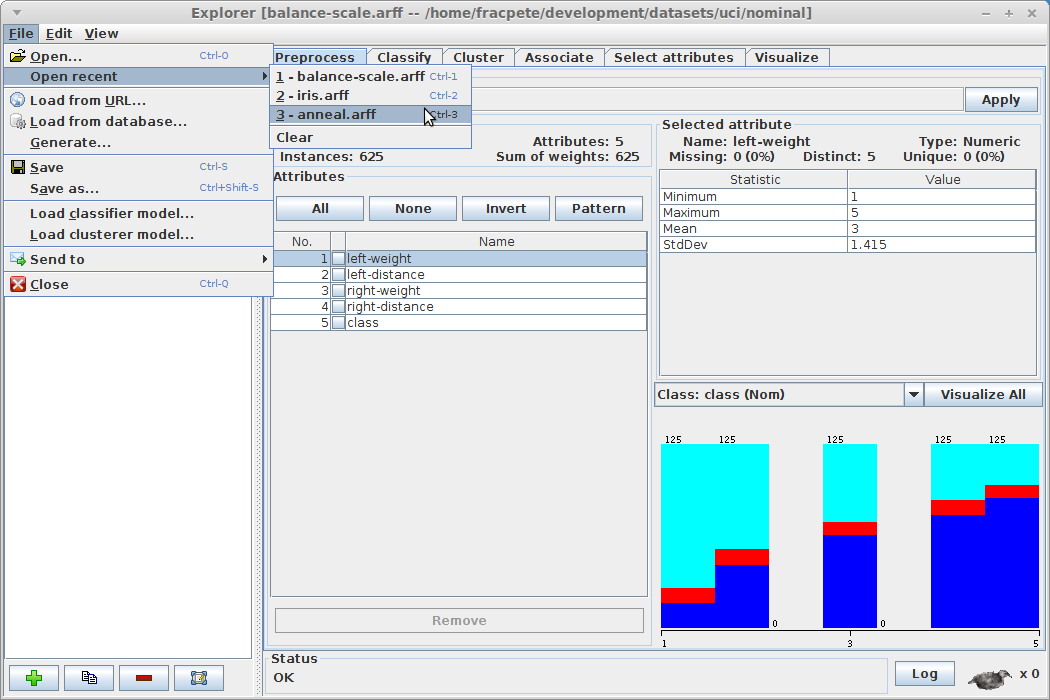
\includegraphics[width=12.0cm]{images/explorerext.png}
  \caption{Explorer interface with menus.}
  \label{explorerext}
\end{figure}

One very useful feature is the notion of \textit{workspaces} in this interface.
You can save the current setup (current dataset, classifiers, clusterers,
evaluation set up, results, etc.) to a file and restore all of it in one go
again. Unfortunately, not all data can be stored, such as the log, the undo
history and the built models or visualizations associated with a results.
See Figure \ref{explorerext-workspaces} for the button (highlighted in red)
that allows you to load/save workspaces.

\begin{figure}[htb]
  \centering
  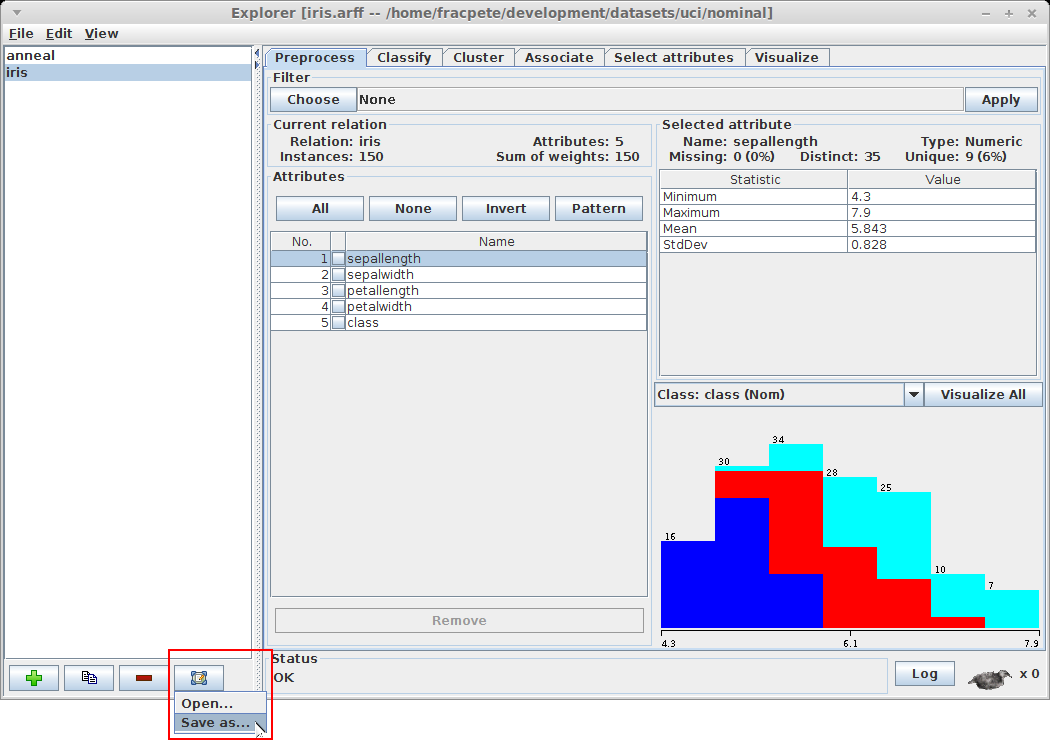
\includegraphics[width=12.0cm]{images/explorerext-workspaces.png}
  \caption{Saving/restoring of workspaces.}
  \label{explorerext-workspaces}
\end{figure}

\clearpage
\section{Hermione}
The \textit{Hermione} wizard allows you to set up and monitor a genetic
algorithm that determines the best parameter settings, based on the classifier
and metric you choose to optimize on. The output directory that you define
(see Figure \ref{hermione_setup}), is used to store all the setups/datasets
that improved the metric. The optimization can be paused, resumed or
stopped with the buttons at the bottom right of the view panel (see Figure
\ref{hermione_run}).

\begin{figure}[htb]
  \centering
  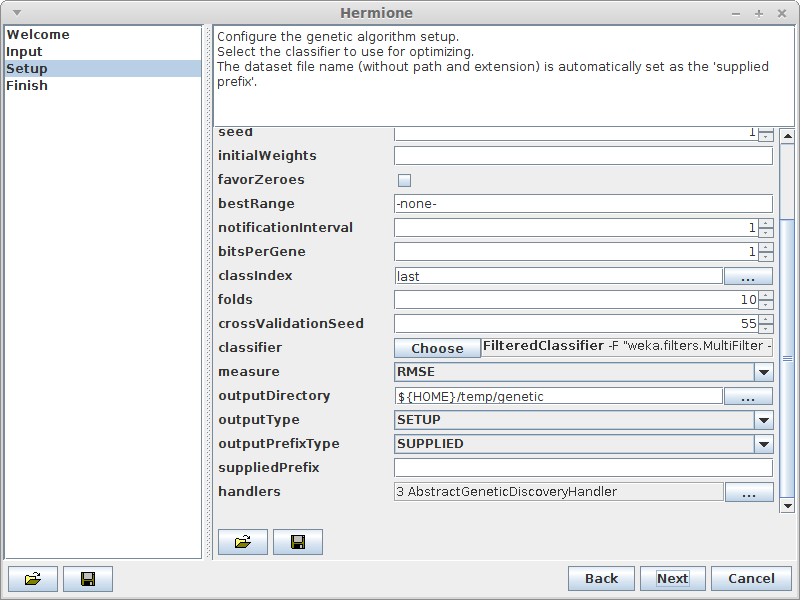
\includegraphics[width=12.0cm]{images/hermione_setup.png}
  \caption{Hermione setup.}
  \label{hermione_setup}
\end{figure}

\begin{figure}[htb]
  \centering
  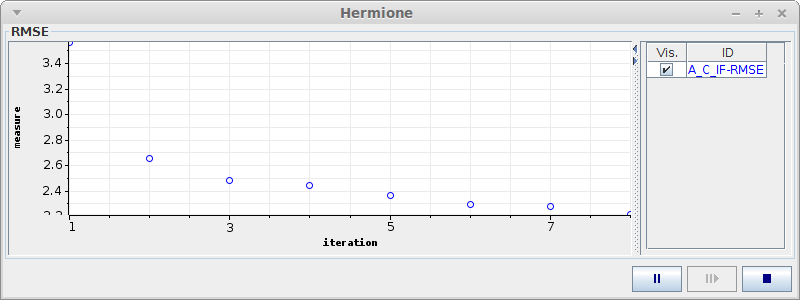
\includegraphics[width=12.0cm]{images/hermione_run.png}
  \caption{Hermione run.}
  \label{hermione_run}
\end{figure}

\clearpage
\section{Investigator}
The \textit{Weka Investigator} (see Figure \ref{wekainvestigator}) is aimed
to be a replacement of the Weka Explorer. The idea is to have a more versatile
and efficient user interface: manage multiple sessions, each session can manage
multiple datasets (e.g., train and test set), making use of tabs instead of windows
(but output tabs can still be detached for comparison), configuration of
outputs to generate each time an evaluation is run (statistics, model,
classifier errors, etc).

\begin{figure}[htb]
  \centering
  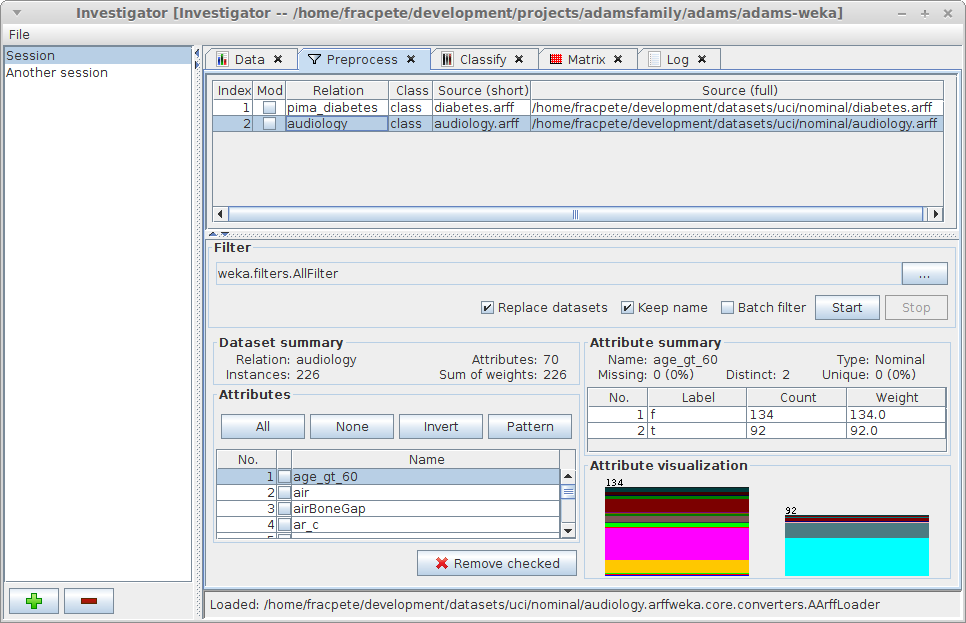
\includegraphics[width=12.0cm]{images/wekainvestigator.png}
  \caption{Weka Investigator.}
  \label{wekainvestigator}
\end{figure}

\clearpage
\section{Make compatible datasets}
When dealing with data across multiple spreadsheets, e.g., training, test
and validation set, then it can happen that these datasets are not compatible
in the strict Weka sense.

The \textit{Make compatible datasets} wizard allows you to turn spreadsheets
into compatible ARFF files:
\begin{tight_itemize}
  \item Select the datasets to make compatible (see \ref{makecompatible1})
  \item Configure how the datasets are being read (see \ref{merge_datasets2})
  \item Select the output directory for the compatible ARFF files (see \ref{merge_datasets3})
  \item Info dialog after processing the datasets (see \ref{merge_datasets4})
\end{tight_itemize}

\begin{figure}[htb]
  \centering
  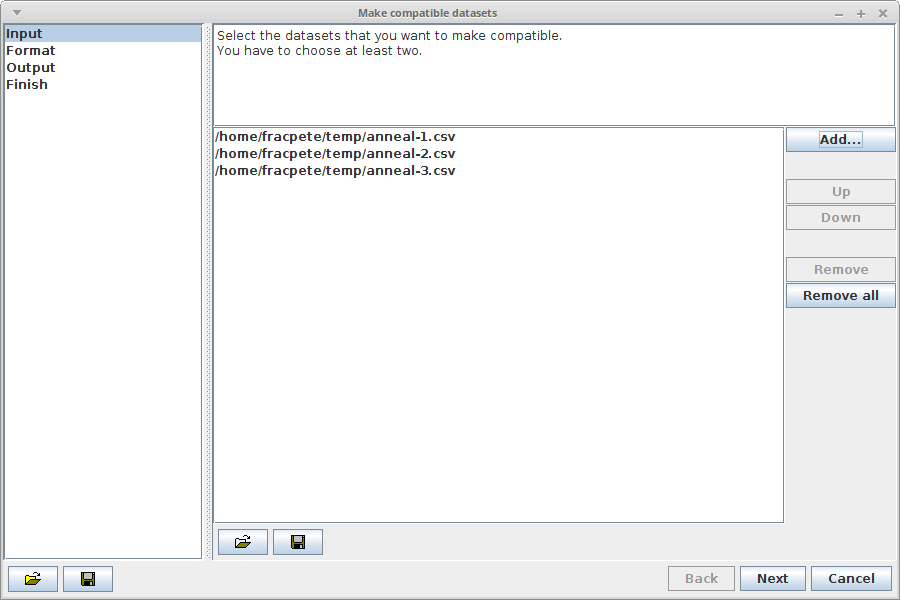
\includegraphics[width=12.0cm]{images/makecompatible1.png}
  \caption{Selecting input files for making compatible datasets.}
  \label{makecompatible1}
\end{figure}

\begin{figure}[htb]
  \centering
  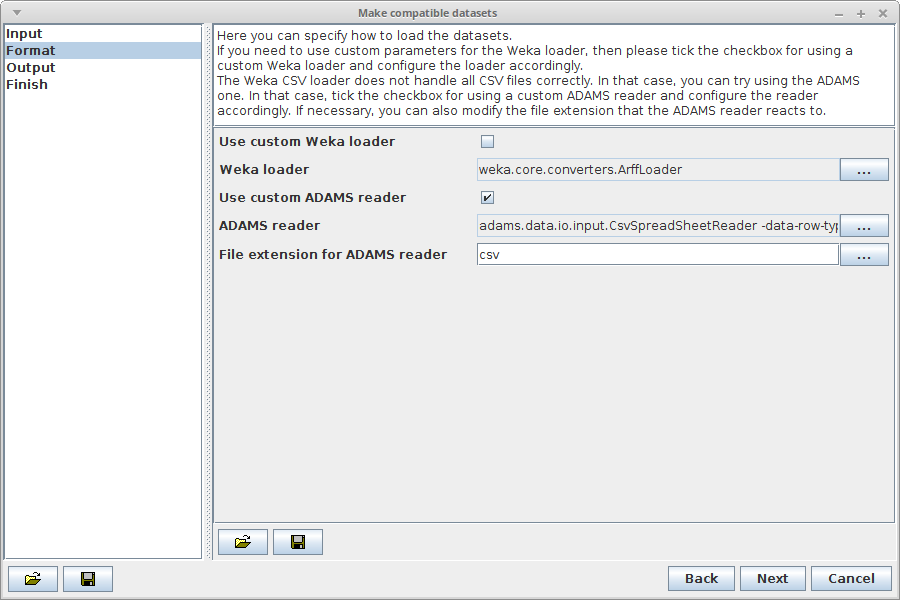
\includegraphics[width=12.0cm]{images/makecompatible2.png}
  \caption{Configuring the readers for the datasets.}
  \label{makecompatible2}
\end{figure}

\begin{figure}[htb]
  \centering
  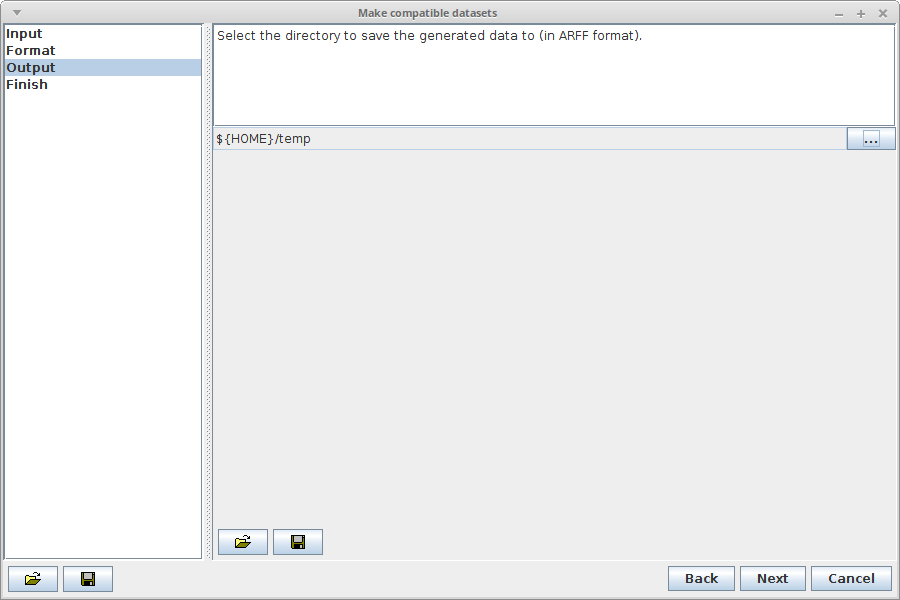
\includegraphics[width=12.0cm]{images/makecompatible3.png}
  \caption{Selecting the output directory for the compatible ARFF files.}
  \label{makecompatible3}
\end{figure}

\begin{figure}[htb]
  \centering
  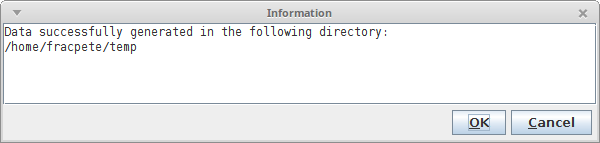
\includegraphics[width=8.0cm]{images/makecompatible4.png}
  \caption{The dialog when dataset generation was successful.}
  \label{makecompatible4}
\end{figure}

\clearpage
\section{Merge datasets}
The process of adding reference data to a dataset or performing
\textit{data fusion}\footnote{\url{https://en.wikipedia.org/wiki/Data_fusion}{}},
can be quite often a manual process, copy/pasting datasets in a spreadsheet
application.

The \textit{Merge datasets} wizard allows you to perform the
process of combining datasets side-by-side conveniently in the GUI:
\begin{tight_itemize}
  \item Select the datasets to merge (see \ref{merge_datasets1})
  \item Configure the merge (see \ref{merge_datasets2})
  \item Select the output file (see \ref{merge_datasets3})
  \item Info dialog after merging (see \ref{merge_datasets4})
\end{tight_itemize}
Figure \ref{merge_datasets-output} shows an example of a merged file.

\begin{figure}[htb]
  \centering
  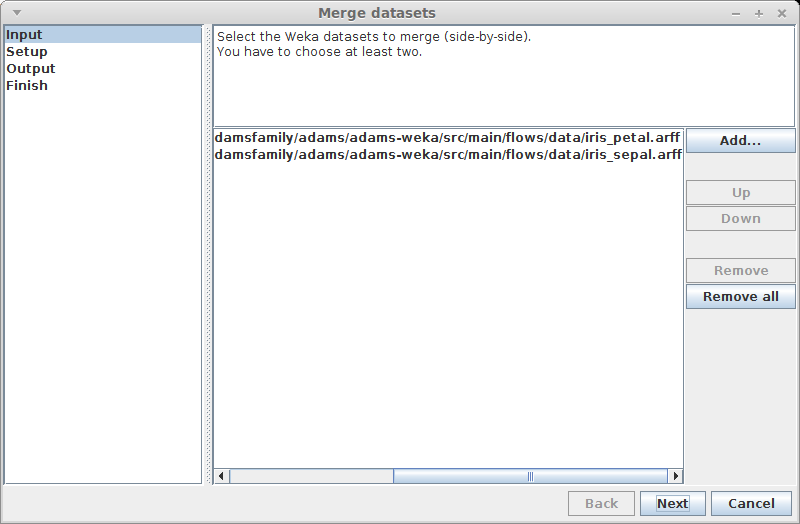
\includegraphics[width=12.0cm]{images/merge_datasets1.png}
  \caption{Selecting input files for merging.}
  \label{merge_datasets1}
\end{figure}

\begin{figure}[htb]
  \centering
  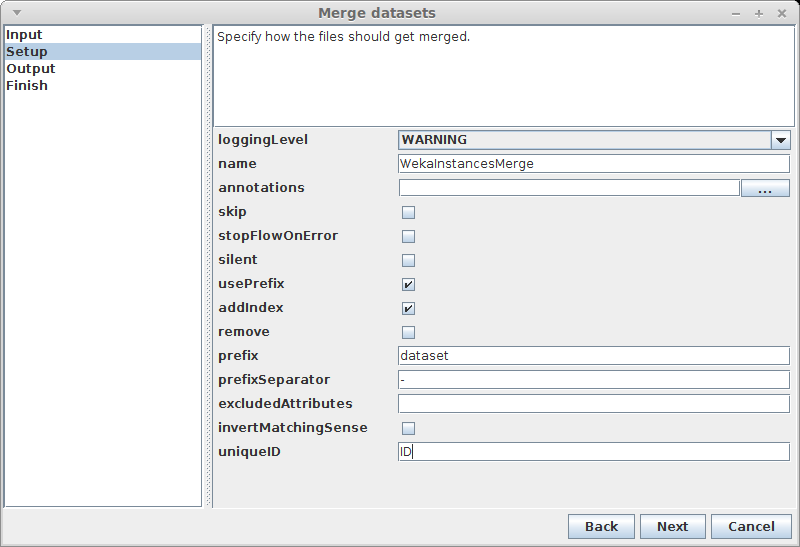
\includegraphics[width=12.0cm]{images/merge_datasets2.png}
  \caption{Configuring the merge.}
  \label{merge_datasets2}
\end{figure}

\begin{figure}[htb]
  \centering
  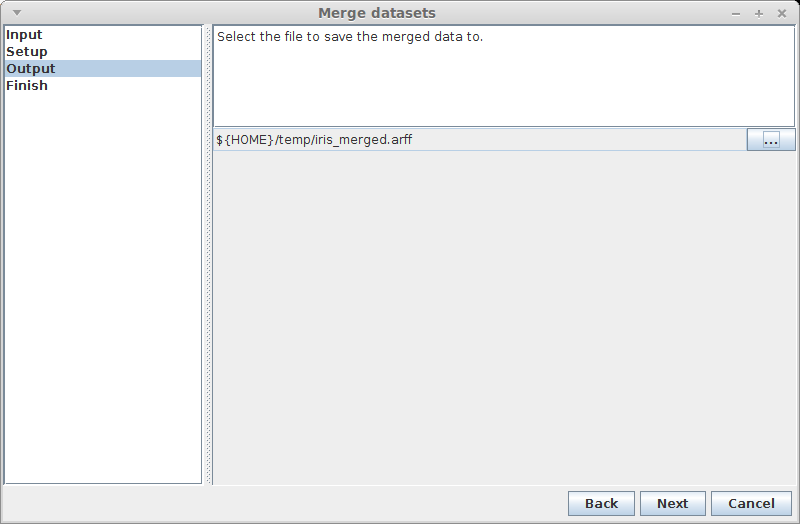
\includegraphics[width=12.0cm]{images/merge_datasets3.png}
  \caption{Selecting the output directory for the filtered datasets.}
  \label{merge_datasets3}
\end{figure}

\begin{figure}[htb]
  \centering
  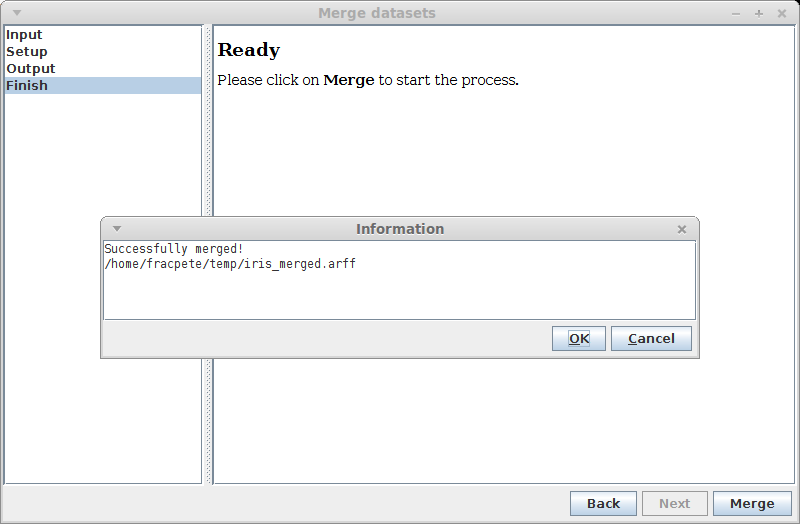
\includegraphics[width=12.0cm]{images/merge_datasets4.png}
  \caption{The dialog when merging was successful.}
  \label{merge_datasets4}
\end{figure}

\begin{figure}[htb]
  \centering
  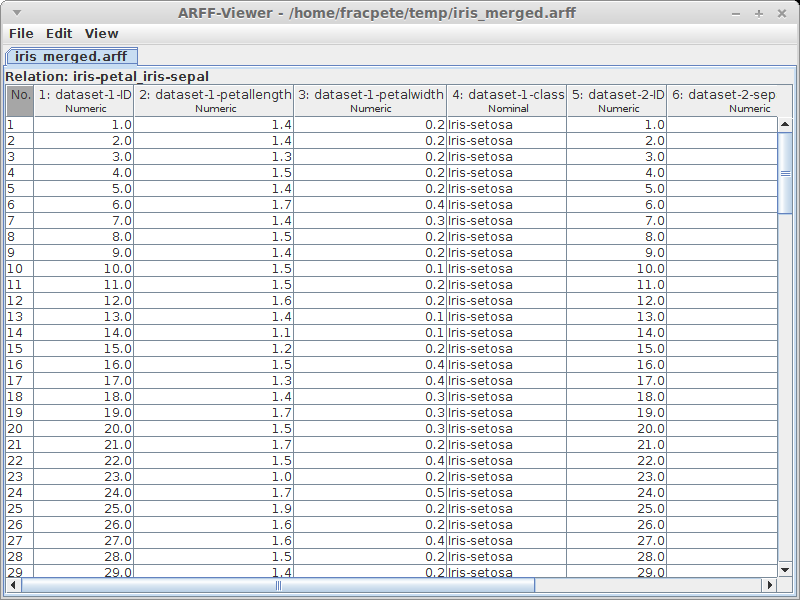
\includegraphics[width=12.0cm]{images/merge_datasets-output.png}
  \caption{The merged dataset.}
  \label{merge_datasets-output}
\end{figure}

\clearpage
\section{Workbench}
The more flexible alternative to the Explorer is called the \textit{Workbench}.
A screenshot is shown in Figure \ref{workbench}.

\begin{figure}[htb]
  \centering
  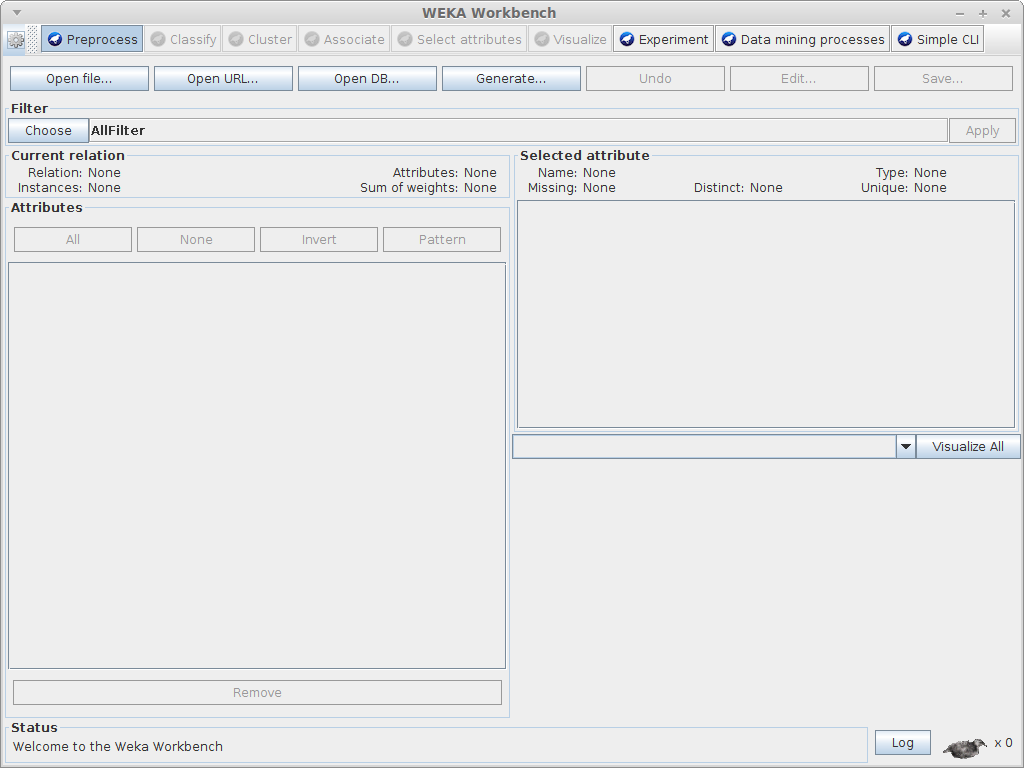
\includegraphics[width=12.0cm]{images/workbench.png}
  \caption{The Workbench interface.}
  \label{workbench}
\end{figure}
